\setcounter{chapter}{-1} % Para empezar a contar en 0

\chapter{Introducción}

La mayoría de ecuaciones diferenciales han sido planteadas por campos como la física. Veamos el caso de un péndulo:

\begin{figure}[H]
    \centering
    \begin{subfigure}{0.3\textwidth}
        \centering        
        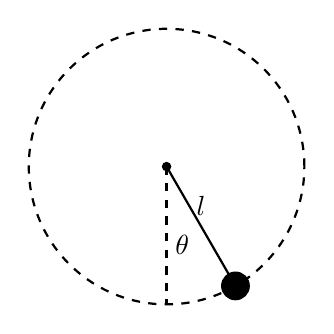
\begin{tikzpicture}
            \centering

            \def\radius{1.75}
            \def\angulo{150}

            % Desactiva los caracteres conflictivos
            \shorthandoff{>} % Para poner puntas de flecha

            \draw[thick, dashed] (0,0) circle (\radius);
            \filldraw (0,0) circle (1.5pt);
            \filldraw ({sin(\angulo)*\radius}, {cos(\angulo)*\radius}) circle (5pt);
            \draw[thick] (0,0) -- ({sin(\angulo)*\radius}, {cos(\angulo)*\radius}) node[midway, above] {$l$};
            \draw[thick, dashed] (0,0) -- (0,-\radius);
            \node at (0.2,-1) {$\theta$};

        \end{tikzpicture}

        \vspace*{0.25cm}
    \end{subfigure}
    \hfill
    \begin{subfigure}{0.6\textwidth}%
        Las condiciones que definen el péndulo son $g >0$, ya que se encuentra en la Tierra, $l$ que es la longitud del péndulo y $\theta$ que es el ángulo con respecto a la vertical.

        La ecuación que define el ángulo a lo largo del tiempo es la siguiente:
        \begin{gather*}
            \theta''(t) + \frac{g}{l} \sen(\theta(t)) = 0
        \end{gather*}
    \end{subfigure}
    \hfill
\end{figure}

Esta es una ecuación diferencial de segundo orden (ya que aparece una segunda derivada). En ella tenemos que $t$ es la variable independiente y $\theta$ es la incógnita o variable dependiente (que es una función).

Si estudiamos las soluciones de esta ecuación tenemos 
\begin{align*}
    \theta(t) &= 0, \ t\in \bb{R} \text{ es una solución (trivialmente)}\\
    \theta(t) & =\pi, \ t \in \bb{R} \text{ es también solución}\\
    \theta(t) & =2n\pi,\ \theta(t) =n\pi, \ t \in \bb{R},\ n \in \bb{Z} \text{ son infinitas soluciones}\\
\end{align*}

De esta forma podemos ver que una ecuación diferencial puede tener infinitas soluciones.

\begin{definicion}
    Podemos definir una \textbf{ecuación diferencial de primer orden} como la relación funcional dada por 
    \begin{gather*}
        \Phi (t, x(t), x'(t)) = 0
    \end{gather*}
    donde $t$ es la \textbf{variable independiente} y $x=x(t)$ es la \textbf{variable independiente} o \textbf{incógnita}.
\end{definicion}

\begin{ejemplo}
    Consideremos la ecuación diferencial dada por
    \begin{gather*}
        x(t) + x'(t)^2 = 1
    \end{gather*}
    Podemos definir\footnote{Notación física} $\Phi = \Phi(t,x,y) = x^2 + y^2 -1$, o equivalentemente\footnote{Notación moderna (matemática)}
    \begin{align*}
        \Phi : D \subset \bb{R}^3 &\rightarrow \bb{R} \\
        (t,x,y) & \mapsto \Phi(t,x,y) = x^2 + y^2 -1
    \end{align*}
    Estudiemos las soluciones a esta ecuación:

    \begin{figure}[H]
        \centering
        
        \begin{subfigure}{0.3\textwidth}
            \centering
            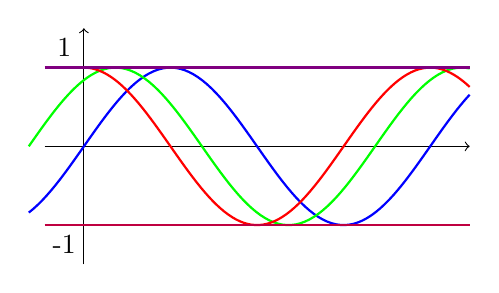
\begin{tikzpicture}
                % Desactiva los caracteres conflictivos
                \shorthandoff{>} % Para poner puntas de flecha

                \def\escalax{0.7}
                % Ejes
                \draw[->] (-0.5,0) -- (\escalax*7,0);
                \draw[->] (0,-1.5) -- (0,1.5);
            
                % Gráfica del seno
                \draw[blue, thick, domain=-1:7, samples=100] plot (\escalax*\x,{sin(\x r)});

                % Gráfica del seno trasladada
                \draw[green, thick, domain=-1:7, samples=100] plot (\escalax*\x,{sin(((\x+1) r))});
            
                % Gráfica del coseno
                \draw[red, thick, domain=0:7, samples=100] plot (\escalax*\x,{cos(\x r)});

                % Horizontales
                \draw[violet, thick] (-0.5,1) --(\escalax*7,1);
                \draw[purple, thick] (-0.5,-1) --(\escalax*7,-1);
            
                    
                % Etiquetas de los valores en el eje y
                \node at (-0.25,1.25) {1};
                \node at (-0.25,-1.25) {-1};
            \end{tikzpicture}

            \vspace*{0.5cm}
    
        \end{subfigure}
        \hfill
        \begin{subfigure}{0.6\textwidth}%
            \begin{itemize}
                \item[\textcolor{blue}{$\bullet$}] $x(t) = \sen(t)$, $t \in \bb{R}$
                \item[\textcolor{red}{$\bullet$}] $x(t)= \cos(t)$, $t \in \bb{R}$
                \item[\textcolor{violet}{$\bullet$}] $x(t)=1$, $t \in \bb{R}$
                \item[\textcolor{purple}{$\bullet$}] $x(t)=-1$, $t \in \bb{R}$
                \item[\textcolor{green}{$\bullet$}] $x(t)=\sen(t+c)$, $t \in \bb{R}$ $\forall c \in \bb{R}$ (familia uniparamétrica).
            \end{itemize}
        \end{subfigure}
        \hfill
    \end{figure}

    Podemos construir otra solución uniendo las ya dadas como por ejemplo
    \begin{gather*}
        x(t)=\left\{
        \begin{array}{ccc}
            \cos(t)& \text{ si }& t \geq 0\\
            1&  \text{ si } & t <0
        \end{array}
        \right.
    \end{gather*}
    Esta función es derivable y por tanto solución a la ecuación.

\end{ejemplo}

Típicamente estudiaremos ecuaciones diferenciales de primer orden en \textbf{forma normal}, es decir, ecuaciones que se pueden escribir como
\begin{gather*}
    x'(t) = f(t, x(t))
\end{gather*}
Esto es una subfamilia de las ecuaciones previamente descritas.